% !TEX root=/home/tavant/these/manuscript/src/manuscript.tex

\section{Full dielectric model }
  \label{sec-fulldiel}
  
  We have observed the effects of the electron emission and the electrostatic boundary condition separately in \cref{sec-diel_layer} and \cref{sec-see} respectively.
  In this section, we investigate the interaction between the two phenomena of the dielectric walls.
  
  
  In \Cref{sec-see}, we observed three regimes depending on the emission rate.
  At high emissivity, the sheath is space-charge limited, resulting in an inverse sheath.
  At low emissivity, we obtain the standard sheath model with electron emission.
  The transition between the regimes passes by a oscillating regime.
  
  \Cref{sec-diel_layer} showed that when there is no emission, the dielectric boundary condition for the potential do not change the simulation results.
  Hence, we chose to investigate the interaction when the emission is high.
  More precisely, the second regime is the most interesting, as it feature a complex behavior.
  
  \begin{figure}[hbtp]
    \centering
    \begin{tabular}{c c}
      \subfigure{see_diel_temporal}{a}{20,20} & 
      \subfigure{see_diel_space}{b}{20,20}
    \end{tabular}
    \caption{Comparison of the ({\bf a}) temporal and ({\bf b}) spatial evolution of the radial electric field at the wall compared to the surface charge. }
    \label{fig-seediel_Er}
  \end{figure}
   
  \Cref{fig-seediel_Er} shows the ({\bf a}) temporal and ({\bf b}) spatial evolution of the radial electric field at the wall compared to the surface charge, similarly  to \cref{fig-er_time}.{\bf b}.
  We can see that in contrast to the results of \cref{sec-diel_layer}, the two values are significantly different.
  The electric field measured in the simulation is rather uniform and constant, compared to the surface charge.
  
  Moreover, in \cref{fig-seediel_Er}.{\bf a}, we see that at around $t=2.1\,\second$, the electric field sign changes, meaning that the sheath passes from the \ac{SCL} regime to the normal regime.
  However, the surface charge is not consistent with this change of regime.
  
  
  \begin{figure}[hbtp]
    \centering
    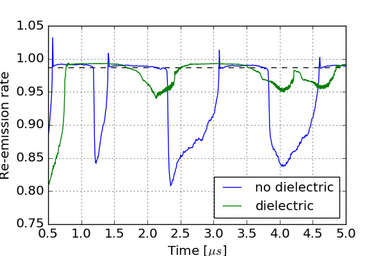
\includegraphics[width=\defaultwidth]{see_RSO}
    \caption{Temporal evolution of the mean electron emission rate $\ratepic$ for the same parameter $\crover=45\,\volt$, with and without the dielectric layer modeled.}
    \label{fig-rso_diel}
  \end{figure}
  
  \cref{fig-rso_diel} compares the temporal evolution of the mean electron emission rate $\ratepic$ for the same parameter $\crover=45\,\volt$, with and without the dielectric layer modeled.
  We see that the oscillations happens for the two models.
  However, we can observe several differences.
  The first is the lower level of emission rate.
  When the wall are grounded, $\ratepic$ decreases at around $85\%$.
  On the contrary, with the dielectric layer included, the emission rate do not decrease much below $95\%$.
  This results in a different overall mean emission rate, that can affect the particle and power balances, hence the mean electron temperature and the performance and the thruster.
  
  
  
  
  